\section{摩擦起电 两种电荷}\label{sec:7-1}

\begin{wrapfigure}{r}{7cm}
    \centering
    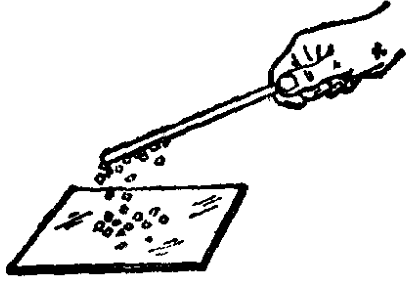
\includegraphics[width=6cm]{../pic/czwl2-ch7-1}
    \caption{丝绸摩擦过的玻璃棒能吸引纸屑}\label{fig:7-1}
\end{wrapfigure}

公元前六世纪的时候,古希腊人发现用毛皮或毛织物摩擦过的琥珀,能够吸引羽毛、头发等轻小物体。
两千多年之后,到十六世纪初,人们进一步知道,不仅毛皮摩擦过的琥珀有这种性质,丝绸摩擦过的玻璃棒,
毛皮摩擦过的硬橡胶棒,绒布摩擦过的硫磺块等,都有这种性质(图 \ref{fig:7-1})。


\CJKunderwave{物体有了吸引轻小物体的性质,我们就说物体带了电,或者说带了电荷}。
用摩擦的方法使物体带电叫做摩擦起电。

摩擦起电的现象在日常生活里也可以看到。
例如,在空气干燥的时候,用塑料梳子梳干净的头发,头发会随着梳子飘起来,
就是因为梳子带了电,吸引头发的缘故。

\begin{figure}[htbp]
    \centering
    \begin{minipage}{7cm}
    \centering
    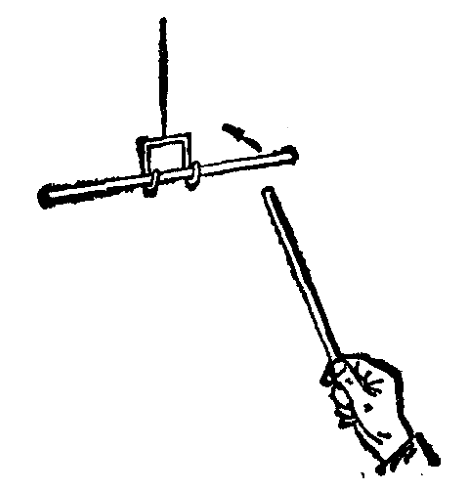
\includegraphics[width=5cm]{../pic/czwl2-ch7-2}
    \caption{}\label{fig:7-2}
    \end{minipage}
    \qquad
    \begin{minipage}{7cm}
    \centering
    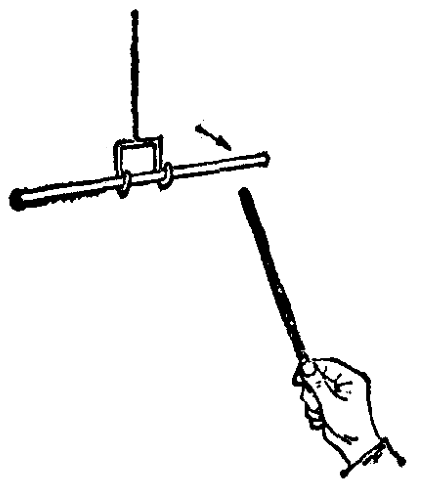
\includegraphics[width=5cm]{../pic/czwl2-ch7-3}
    \caption{}\label{fig:7-3}
    \end{minipage}
\end{figure}

人们研究摩擦起电现象时还发现:用绸子摩擦过的两根玻璃棒互相推斥(图 \ref{fig:7-2}),
用毛皮摩擦过的两根橡胶棒也互相推斥;
但是用绸子摩擦过的玻璃棒跟用毛皮摩擦过的橡胶棒互相吸引(图 \ref{fig:7-3})。
这个现象使人们认识到,用绸子摩擦过的玻璃棒上带的电跟用毛皮摩擦过的橡胶棒上带的电是不同的。
人们用各种各样的物质互相摩擦带电后,发现
凡是跟绸子摩擦过的玻璃棒吸引的,必定跟毛皮摩擦过的橡胶棒推斥;
凡是跟毛皮摩擦过的橡胶棒吸引的,必定跟绸子摩擦过的玻璃棒推斥。
这些事实使人们认识到\CJKunderwave{自然界中只存在两种电荷}。

人们把用绸子摩擦过的玻璃棒带的电荷叫做\textbf{正电荷},
     用毛皮摩擦过的橡胶棒带的电荷叫做\textbf{负电荷}。

\textbf{同种电荷互相推斥,异种电荷互相吸引}。

利用电荷间的相互作用,人们制成了检验物体带不带电的仪器——验电器。
带电体接触验电器的金属球的候(图 \ref{fig:7-4}),就有一部分电荷转移到验电器的两片金属箔上,
这两片金属箔由于带同种电荷互相推斥而张开。
我们从金属箔的张开可以断定跟金属球接触的物体是带电的。

\begin{figure}[htbp]
    \centering
    \begin{minipage}{7cm}
    \centering
    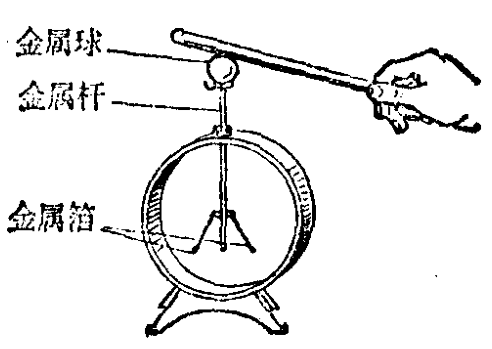
\includegraphics[width=6cm]{../pic/czwl2-ch7-4}
    \caption{}\label{fig:7-4}
    \end{minipage}
    \qquad
    \begin{minipage}{7cm}
    \centering
    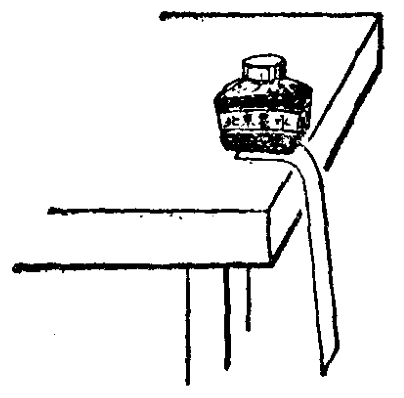
\includegraphics[width=5cm]{../pic/czwl2-ch7-5}
    \caption{}\label{fig:7-5}
    \end{minipage}
\end{figure}

\section*{小实验}

剪一些碎纸屑。从塑料薄膜上剪下 20 厘米长、2 厘米宽的两条。

把一条塑料薄膜铺在桌面上,用手帕(或丝绸)在薄膜上摩擦几下,然后利用纸屑检查薄膜条是不是带了电。

把带了电的薄膜条上端压在桌边上(图 \ref{fig:7-5})。

用手帕摩擦另一条塑料薄膜,然后把这条塑料薄膜拿近压在桌边的那一条,看到了什么现象?为什么?

把手帕拿近压在桌边的薄膜条,看到了什么现象?为什么?

